\documentclass[11pt,a4paper]{article}

%------------------------------------------------
% Packages and formatting
%------------------------------------------------
%================================================
% Page layout
%================================================

\usepackage[
    a4paper,
    margin=2.5cm
]{geometry}

%================================================
% Mathematics
%================================================

\usepackage{amsmath}
\usepackage{amssymb}
\usepackage{amsfonts}
\usepackage{bm}

%================================================
% Figures and tables
%================================================

\usepackage{graphicx}
\usepackage{float}
\usepackage{subcaption}
\usepackage{booktabs}
\usepackage{caption}
\usepackage{tabularx}

%================================================
% Fonts and typography
%================================================

\usepackage[T1]{fontenc}
\usepackage{lmodern}

\usepackage{setspace}
\setstretch{1.1}

\setlength{\parindent}{0pt}
\setlength{\parskip}{0.6em}

%================================================
% Section formatting
%================================================

\usepackage{titlesec}

\titleformat{\section}
{\Large\bfseries}
{\thesection.}
{0.6em}
{}

\titleformat{\subsection}
{\large\bfseries}
{\thesubsection}
{0.6em}
{}

\titlespacing*{\section}
{0pt}{18pt}{10pt}

\titlespacing*{\subsection}
{0pt}{12pt}{6pt}

%================================================
% Hyperlinks
%================================================

\usepackage[
colorlinks=true,
linkcolor=blue,
citecolor=blue,
urlcolor=blue
]{hyperref}

%================================================
% Header and footer
%================================================

\usepackage{fancyhdr}

\pagestyle{fancy}

\fancyhf{}

\fancyhead[L]{CFD Portfolio}
\fancyhead[R]{Project 01}

\fancyfoot[C]{\thepage}

\renewcommand{\headrulewidth}{0.4pt}

\setlength{\headheight}{25pt}
\setlength{\headsep}{25pt}

%================================================
% Lists
%================================================

\usepackage{enumitem}

\setlist{
itemsep=3pt,
topsep=5pt
}

%================================================
% Figure captions
%================================================

\captionsetup{
font=small,
labelfont=bf
}
\renewcommand{\arraystretch}{0.9}
\setlength{\abovecaptionskip}{4pt}
\setlength{\belowcaptionskip}{4pt}
\setlength{\intextsep}{8pt}

%================================================
% Table spacing
%================================================

\renewcommand{\arraystretch}{1.25}

%------------------------------------------------
% Document information
%------------------------------------------------

\title{
    \Huge\textbf{Steady Two-Dimensional Heat Conduction}\\[0.4cm]
    \Large
    A Second-Order Finite-Volume Solver using the Point Gauss-Seidel Method
}

\author{
    \Large Arian Shahnoori
}

\date{\today}

%================================================
\begin{document}
%================================================

\maketitle
\thispagestyle{empty}

\vspace{0.8cm}

\begin{abstract}
A two-dimensional finite-volume solver is developed for the steady-state heat conduction equation on a square domain. The Laplace equation is discretized using a second-order cell-centered finite-volume formulation on a structured Cartesian grid and solved iteratively using the Point Gauss-Seidel method. The numerical implementation is verified through comparison with the analytical solution. Several post-processing techniques, including contour plots, line-cut comparisons, error distributions, and residual convergence histories, are employed to assess both the accuracy of the numerical solution and the convergence characteristics of the iterative solver.
\end{abstract}

\vspace{0.5cm}

\begin{center}
\begin{tabular}{ll}
\toprule
Problem & Steady Two-Dimensional Heat Conduction\\
Governing Equation & Laplace Equation\\
Discretization & Cell-Centered Finite Volume Method\\
Spatial Accuracy & Second Order\\
Linear Solver & Point Gauss-Seidel\\
Programming Language & Python\\
Verification & Analytical Solution\\
\bottomrule
\end{tabular}
\end{center}

\newpage

\tableofcontents

\newpage


\section{Introduction}

Heat conduction is one of the three fundamental modes of heat transfer and plays a central role in numerous engineering applications, including thermal management systems, heat exchangers, electronic cooling, and energy systems. While analytical solutions exist for a limited number of idealized problems, most practical engineering applications involve complex geometries, material properties, or boundary conditions that require numerical solution techniques.

Before applying a numerical method to complex engineering problems, it is essential to verify that the numerical implementation correctly reproduces solutions for cases where an analytical solution is available. Code verification provides confidence that the governing equations, boundary conditions, spatial discretization, and numerical solution algorithms have been implemented correctly.

The objective of this project is to develop a numerical solver for the two-dimensional steady-state heat conduction equation on a square domain. The governing equation is discretized using a second-order finite-volume formulation on a structured Cartesian mesh and solved iteratively using the Point Gauss-Seidel method. The numerical solution is verified through direct comparison with the corresponding analytical solution of the Laplace equation.

Beyond validating the numerical implementation, this project establishes a reusable computational framework for future developments, including mesh refinement studies, accelerated iterative methods such as Successive Over-Relaxation (SOR), and more advanced computational fluid dynamics applications.



\section{Governing Equation}

The physical problem considered in this study is two-dimensional steady-state heat conduction in a square domain with no internal heat generation. Under these assumptions, the conservation of energy reduces to the Laplace equation,

\begin{equation}
\nabla^2 T
=
\frac{\partial^2 T}{\partial x^2}
+
\frac{\partial^2 T}{\partial y^2}
=
0
\label{eq:laplace}
\end{equation}

where $T$ denotes the temperature field and $x$ and $y$ are the Cartesian spatial coordinates.

The computational domain and the prescribed boundary conditions are illustrated in Figure~\ref{fig:domain}. Dirichlet boundary conditions are imposed on all boundaries, meaning that the temperature is explicitly prescribed along the boundaries of the computational domain. These boundary conditions uniquely determine the solution of Equation~\ref{eq:laplace}.

\begin{figure}[H]
    \centering
    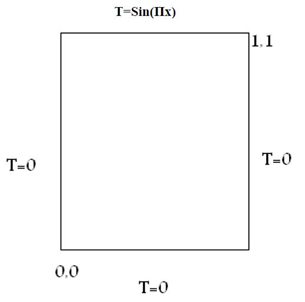
\includegraphics[width=0.4\textwidth]{figures/domain.png}
    \caption{Computational domain and prescribed boundary conditions.}
    \label{fig:domain}
\end{figure}

For the selected boundary conditions, an analytical solution exists and can therefore be used to verify the numerical implementation. The exact solution of Equation~\ref{eq:laplace} is

\begin{equation}
T(x,y)
=
\frac{\sin(\pi x)\sinh(\pi y)}
{\sinh(\pi)}
\label{eq:exact}
\end{equation}

The existence of the analytical solution given by Equation~\ref{eq:exact} makes this problem an ideal verification benchmark. Throughout this project, the numerical solution obtained using the finite-volume discretization and the Point Gauss-Seidel iterative solver is compared directly with the analytical temperature distribution to assess the correctness and accuracy of the numerical implementation.



\section{Finite-Volume Discretization}

The governing equation was discretized using the finite-volume method on a structured Cartesian mesh. In this approach, the computational domain is divided into a collection of non-overlapping control volumes, and the governing equation is enforced over each control volume individually. Unlike finite-difference methods, which approximate the governing equation directly at discrete points, the finite-volume method is derived from the integral form of the conservation law, thereby ensuring local conservation within every control volume.

Expressing the Laplace operator in divergence form and integrating over an arbitrary control volume yields

\begin{equation}
\iint_{CV}\nabla\cdot\left(\nabla T\right)\,dA=0
\label{eq:fvm_integral}
\end{equation}

Applying the divergence theorem converts the volume integral into a surface integral over the control-volume boundary,

\begin{equation}
\oint_{CS}\nabla T\cdot\mathbf{n}\,ds=0
\label{eq:gauss}
\end{equation}

where $\mathbf{n}$ denotes the outward unit normal vector to the control surface. Equation~\ref{eq:gauss} states that, at steady state and in the absence of internal heat generation, the net diffusive heat flux through the boundary of every control volume is zero.

The computational stencil and notation adopted throughout the discretization procedure are illustrated in Figure~\ref{fig:grid}.

\begin{figure}[H]
    \centering
    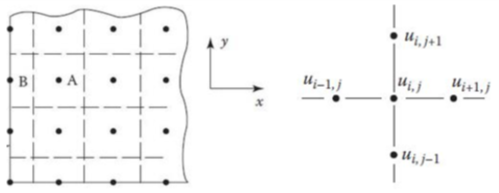
\includegraphics[width=0.60\textwidth]{figures/grid.png}
    \caption{Computational stencil and control-volume notation used in the finite-volume discretization.}
    \label{fig:grid}
\end{figure}

To achieve second-order spatial accuracy, the temperature gradients at the control-volume faces are approximated using central differences. For a uniform Cartesian mesh, the temperature gradient at the east face of a control volume is approximated by

\begin{equation}
\left.\frac{\partial T}{\partial x}\right|_{i+\frac12}
=
\frac{T_{i+1}-T_i}{\Delta x}
+
\mathcal{O}(\Delta x^2)
\label{eq:face_gradient}
\end{equation}

An analogous expression is obtained for the remaining control-volume faces in both coordinate directions.

Substituting the face-gradient approximations into Equation~\ref{eq:gauss} and evaluating the fluxes across the four faces of each control volume yields the discrete form of the governing equation,

\begin{equation}
\frac{T_{i+1,j}-2T_{i,j}+T_{i-1,j}}{\Delta x^2}
+
\frac{T_{i,j+1}-2T_{i,j}+T_{i,j-1}}{\Delta y^2}
=
0
\label{eq:laplace_discrete}
\end{equation}

For the present study, a uniform Cartesian mesh is employed such that

\[
\Delta x=\Delta y.
\]

Under this condition, Equation~\ref{eq:laplace_discrete} provides a second-order accurate approximation of the continuous Laplace equation throughout the computational domain.

The resulting system of algebraic equations is coupled through the neighboring control-volume temperatures and therefore cannot be solved independently for each cell. An iterative solution procedure is consequently required to obtain the numerical temperature distribution.



\section{Numerical Solution Method}

\subsection{Point Gauss-Seidel Iteration}

The finite-volume discretization presented in the previous section results in a coupled system of algebraic equations involving the temperatures of neighboring control volumes. For large systems, iterative methods are generally preferred over direct solution techniques because of their lower memory requirements and straightforward implementation.

In the present work, the Point Gauss-Seidel method is employed to solve the discrete system. Rearranging Equation~\ref{eq:laplace_discrete} to isolate the unknown temperature at the current control volume yields the iterative update equation

\begin{equation}
T_{i,j}^{k+1}
=
\frac{\Delta y^2}{2(\Delta x^2+\Delta y^2)}
\left(
T_{i+1,j}^{k}
+
T_{i-1,j}^{k+1}
\right)
+
\frac{\Delta x^2}{2(\Delta x^2+\Delta y^2)}
\left(
T_{i,j+1}^{k}
+
T_{i,j-1}^{k+1}
\right)
\label{eq:gs}
\end{equation}

where $k$ denotes the iteration number.

Starting from an initial temperature distribution, the solution is updated sequentially throughout the computational domain. As the computation proceeds through the grid, newly computed temperatures immediately replace their values from the previous iteration and are subsequently used when updating neighboring control volumes. This feature distinguishes the Gauss-Seidel method from the Jacobi method and generally results in faster convergence.

The iterative sweep alone is insufficient because the boundary values appearing in Equation~\ref{eq:gs} must also satisfy the prescribed boundary conditions. Consequently, the boundary conditions are updated after every Gauss-Seidel sweep before evaluating convergence.

%%%%%%%%%%%%%%%%%%%%%%%%%%%%%%%%%%%%%%%%%%%%%%%%%%%%%

\subsection{Boundary Condition Implementation}

The numerical formulation employs a cell-centered finite-volume mesh in which temperature values are stored at the centers of the control volumes. Since the physical boundaries do not coincide with computational nodes, the prescribed Dirichlet boundary conditions cannot be imposed directly.

Instead, an additional layer of fictitious control volumes, commonly referred to as ghost cells, is introduced outside the computational domain. Assuming a linear variation of temperature between the neighboring cell centers, the ghost-cell value is obtained from

\begin{equation}
T_b
=
\frac{T_P+T_G}{2},
\qquad
T_G
=
2T_b-T_P
\label{eq:ghost}
\end{equation}

where $T_b$ is the prescribed boundary temperature, $T_P$ denotes the adjacent interior control-volume temperature, and $T_G$ is the ghost-cell temperature.

Updating the ghost cells after every Gauss-Seidel sweep ensures that Equation~\ref{eq:laplace_discrete} remains valid for every interior control volume, including those adjacent to the physical boundaries. This treatment allows a single discretization formula to be applied uniformly throughout the computational domain.

%%%%%%%%%%%%%%%%%%%%%%%%%%%%%%%%%%%%%%%%%%%%%%%%%%%%%

\subsection{Residual Definition}

After each iteration, the accuracy of the current solution is assessed by evaluating the residual of the discrete governing equation. The exact solution satisfies Equation~\ref{eq:laplace_discrete} exactly, whereas any intermediate iterate generally produces a non-zero residual.

For the present problem, the residual associated with each control volume is

\begin{equation}
R_{i,j}
=
\frac{
T_{i+1,j}
+
T_{i-1,j}
+
T_{i,j+1}
+
T_{i,j-1}
-
4T_{i,j}
}
{\Delta x^2}
\label{eq:residual}
\end{equation}

As the iterative solution approaches the exact discrete solution, the residual field tends toward zero throughout the computational domain.

%%%%%%%%%%%%%%%%%%%%%%%%%%%%%%%%%%%%%%%%%%%%%%%%%%%%%

\subsection{Convergence Criterion}

Because every control volume possesses its own residual, convergence is monitored using the norm of the residual field. The general definition of the residual norm is

\begin{equation}
L_p
=
\left(
\frac{
\sum_{i=1}^{N_{\mathrm{CV}}}
A_i
|R_i|^p
}
{
\sum_{i=1}^{N_{\mathrm{CV}}}
A_i
}
\right)^{1/p}
\label{eq:lp}
\end{equation}

where $N_{\mathrm{CV}}$ is the total number of control volumes, $A_i$ is the area of control volume $i$, and $R_i$ is the corresponding residual.

Since all control volumes have identical area in the present structured mesh, Equation~\ref{eq:lp} simplifies to the $L_2$ residual norm,

\begin{equation}
L_2
=
\left(
\frac{
\sum_{i=1}^{N_{\mathrm{CV}}}
R_i^2
}
{N_{\mathrm{CV}}}
\right)^{1/2}
\label{eq:l2}
\end{equation}

The iterative solution procedure is repeated until the $L_2$ residual norm falls below a prescribed convergence tolerance. At this point, the numerical solution is considered converged and the resulting temperature field is used for post-processing and verification against the analytical solution.



\section{Computational Implementation}

The numerical method was implemented in Python using a modular programming structure. Rather than organizing the solver as a single script, the implementation is divided into a collection of independent functions responsible for initialization, boundary-condition treatment, numerical solution, residual evaluation, grid generation, and post-processing. This modular design improves code readability, facilitates debugging, and provides a flexible framework for extending the solver to more advanced numerical methods in future projects.

Table~\ref{tab:functions} summarizes the principal functions comprising the solver.

\begin{table}[H]
\centering
\caption{Major functions of the numerical solver.}
\label{tab:functions}

\begin{tabularx}{\textwidth}{l X}
\toprule
\textbf{Function} & \textbf{Purpose} \\
\midrule

\texttt{initialize\_temperature()} 
& Constructs the initial temperature field and initializes ghost cells around the computational domain. \\

\texttt{apply\_boundary\_conditions()} 
& Updates ghost-cell values to enforce Dirichlet boundary conditions. \\

\texttt{residual\_norm()} 
& Computes the $L_2$ norm of the residual field for convergence monitoring. \\

\texttt{gauss\_seidel()} 
& Performs the iterative Point Gauss-Seidel solution of the discretized Laplace equation. \\

\texttt{create\_grid()} 
& Generates the structured computational grid for post-processing using \texttt{meshgrid}. \\

\texttt{plot\_contours()} 
& Compares numerical and analytical temperature distributions using contour plots. \\

\texttt{plot\_error\_field()} 
& Visualizes the spatial distribution of numerical error. \\

\texttt{plot\_line\_cuts()} 
& Extracts and plots horizontal and vertical temperature profiles for validation. \\

\texttt{plot\_residual\_history()} 
& Displays convergence history as a function of iteration count and computational time. \\

\bottomrule
\end{tabularx}

\end{table}

%%%%%%%%%%%%%%%%%%%%%%%%%%%%%%%%%%%%%%%%%%%%%%%%%%%%%%%%%%%%%

\subsection{Solution Algorithm}

The overall computational procedure consists of the following steps:

\begin{enumerate}
\item Specify the numerical parameters, including the mesh resolution and convergence tolerance.
\item Initialize the computational domain by constructing the temperature field together with the surrounding ghost cells.
\item Apply the prescribed Dirichlet boundary conditions through the ghost-cell values.
\item Repeatedly perform Gauss-Seidel iterations until convergence. Each iteration consists of
    \begin{enumerate}
        \item updating the interior control-volume temperatures,
        \item updating the ghost-cell values,
        \item computing the residual norm, and
        \item checking the convergence criterion.
    \end{enumerate}
\item Construct the computational grid for visualization.
\item Compare the numerical and analytical solutions using contour plots, error distributions, line-cut comparisons, and convergence histories.
\end{enumerate}

%%%%%%%%%%%%%%%%%%%%%%%%%%%%%%%%%%%%%%%%%%%%%%%%%%%%%%%%%%%%%

\subsection{Solver Implementation}

The Point Gauss-Seidel solver receives the initial temperature field, mesh resolution, and convergence tolerance as inputs. During each iteration, the temperatures of all interior control volumes are updated sequentially using Equation~\ref{eq:gs}. After completing one sweep of the computational domain, the ghost-cell values are updated according to Equation~\ref{eq:ghost}. The residual field is subsequently evaluated using Equation~\ref{eq:residual}, and its corresponding $L_2$ norm is computed from Equation~\ref{eq:l2}.

The residual norm, iteration number, and elapsed computation time are stored throughout the solution process to monitor convergence. The iterative procedure terminates once the prescribed convergence tolerance is satisfied, after which the converged temperature field is returned for post-processing.

%%%%%%%%%%%%%%%%%%%%%%%%%%%%%%%%%%%%%%%%%%%%%%%%%%%%%%%%%%%%%

\subsection{Grid Generation}

A structured computational mesh is generated by first constructing one-dimensional arrays containing the coordinates of the control-volume centers in each spatial direction. These arrays are subsequently converted into two-dimensional coordinate matrices using NumPy's \texttt{meshgrid()} function with the \texttt{indexing='ij'} option.

The \texttt{ij} indexing convention preserves the matrix indexing employed throughout the numerical solver such that

\[
X[i,j]=x_i,
\qquad
Y[i,j]=y_j.
\]

Consequently, the temperature field $T[i,j]$ corresponds directly to the physical location $(x_i,y_j)$ without requiring coordinate transposition during visualization. Maintaining this consistent indexing simplifies both the numerical implementation and the post-processing routines.

%%%%%%%%%%%%%%%%%%%%%%%%%%%%%%%%%%%%%%%%%%%%%%%%%%%%%%%%%%%%%

\subsection{Post-Processing}

Several post-processing techniques are employed to evaluate both the accuracy and convergence of the numerical solution.

Contour plots of the numerical and analytical temperature fields provide a qualitative assessment of the overall solution. An error contour illustrates the spatial distribution of the numerical error across the computational domain. Horizontal and vertical line cuts at selected locations enable direct quantitative comparison between the numerical and analytical solutions. Finally, the residual histories plotted as functions of both iteration number and computation time provide insight into the convergence characteristics and computational performance of the Point Gauss-Seidel solver.



\section{Results and Discussion}

\subsection{Temperature Distribution}

Figure~\ref{fig:contours} compares the numerical solution obtained using the finite-volume solver with the analytical solution of the Laplace equation. The two temperature fields exhibit excellent agreement throughout the computational domain. The smooth variation of the temperature contours and the close correspondence between the numerical and analytical solutions demonstrate that the governing equation, spatial discretization, and boundary-condition implementation have been correctly incorporated into the solver.

\begin{figure}[H]
    \centering
    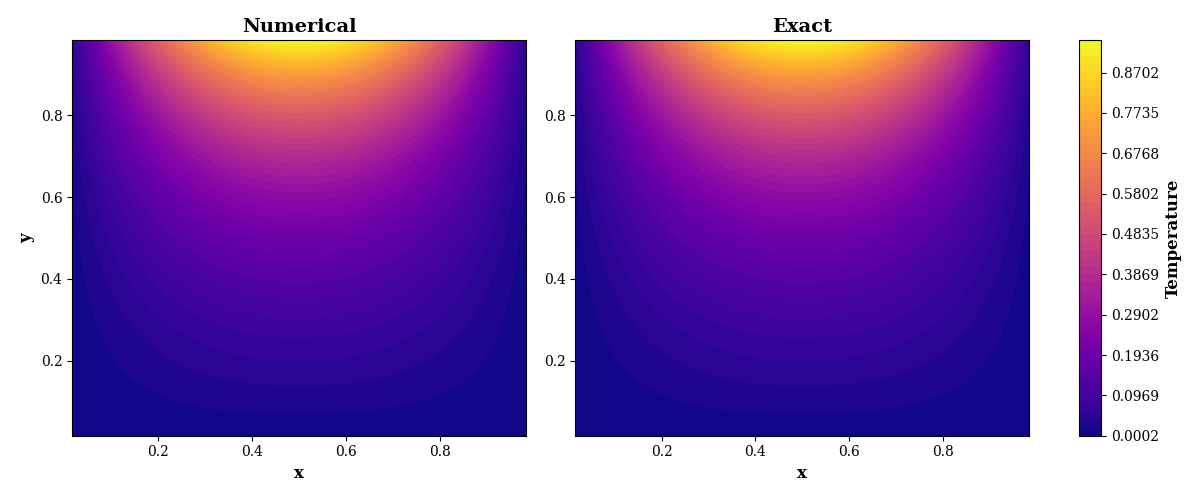
\includegraphics[width=\textwidth]{figures/temperature_contours.png}
    \caption{Comparison of the numerical and analytical temperature distributions.}
    \label{fig:contours}
\end{figure}

%%%%%%%%%%%%%%%%%%%%%%%%%%%%%%%%%%%%%%%%%%%%%%%%%%%%%%%%%%%%%

\subsection{Error Field}

To quantify the numerical accuracy, the pointwise error field was computed as the difference between the analytical and numerical temperature distributions. The resulting error field is shown in Figure~\ref{fig:error}.

The error remains small throughout the computational domain, confirming the second-order accuracy of the spatial discretization. The largest errors occur in regions of relatively large temperature gradients, which is consistent with the expected behavior of finite-volume discretizations on a finite-resolution mesh.

\begin{figure}[H]
    \centering
    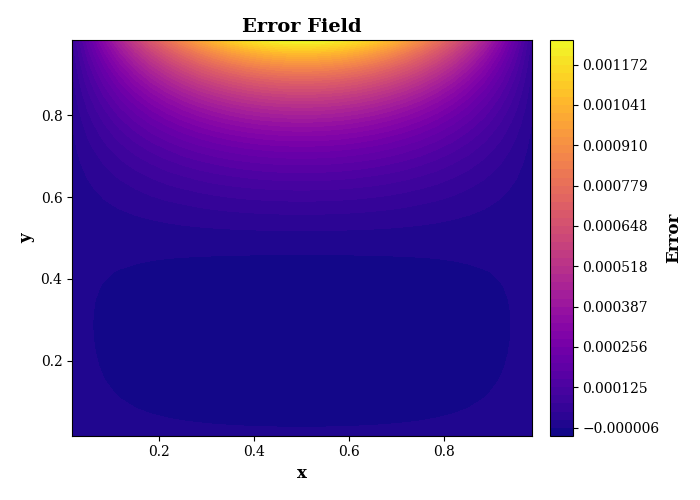
\includegraphics[width=0.65\textwidth]{figures/error_field.png}
    \caption{Spatial distribution of the numerical error.}
    \label{fig:error}
\end{figure}

%%%%%%%%%%%%%%%%%%%%%%%%%%%%%%%%%%%%%%%%%%%%%%%%%%%%%%%%%%%%%

\subsection{Convergence History}

The convergence behavior of the Point Gauss-Seidel solver was monitored using the $L_2$ residual norm. Figure~\ref{fig:residual} presents the residual history as functions of both iteration number and computation time.

The residual decreases monotonically until the prescribed convergence tolerance is satisfied, indicating stable convergence of the iterative solution procedure. The residual-time history additionally provides a useful measure of computational performance and establishes a baseline for future comparisons with accelerated iterative methods such as Successive Over-Relaxation (SOR), Line Gauss-Seidel, ADI, and multigrid methods.

\begin{figure}[H]
    \centering
    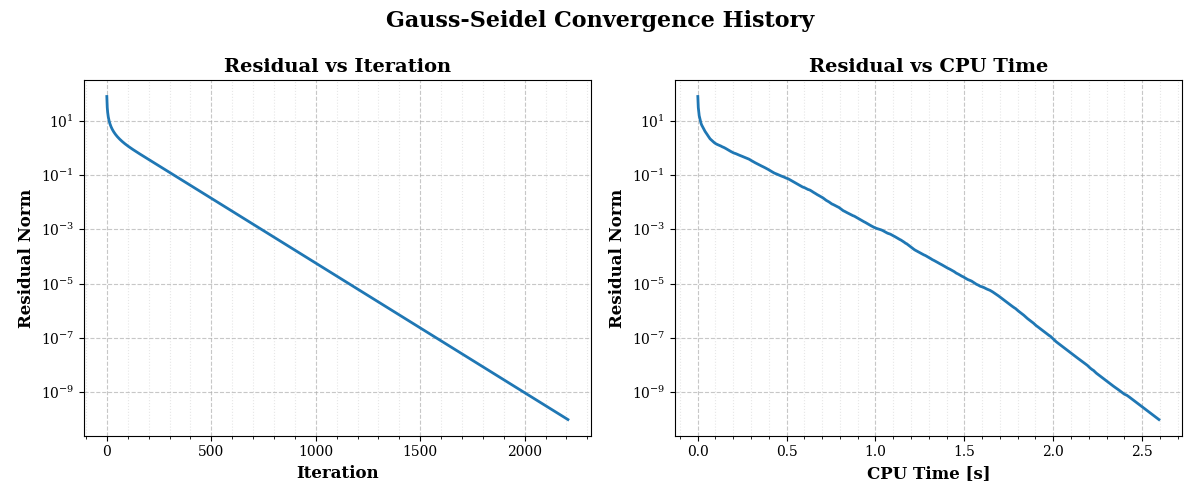
\includegraphics[width=\textwidth]{figures/residual_history.png}
    \caption{Residual convergence histories with respect to iteration count and computation time.}
    \label{fig:residual}
\end{figure}

%%%%%%%%%%%%%%%%%%%%%%%%%%%%%%%%%%%%%%%%%%%%%%%%%%%%%%%%%%%%%

\subsection{Line-Cut Comparison}

To further verify the numerical implementation, horizontal and vertical line cuts were extracted at several locations within the computational domain and compared with the corresponding analytical solution.

As shown in Figure~\ref{fig:linecuts}, the numerical and analytical profiles are nearly indistinguishable for all selected cut locations. The close agreement demonstrates that the solver accurately reproduces both the magnitude and spatial variation of the analytical temperature field.

\begin{figure}[H]
    \centering
    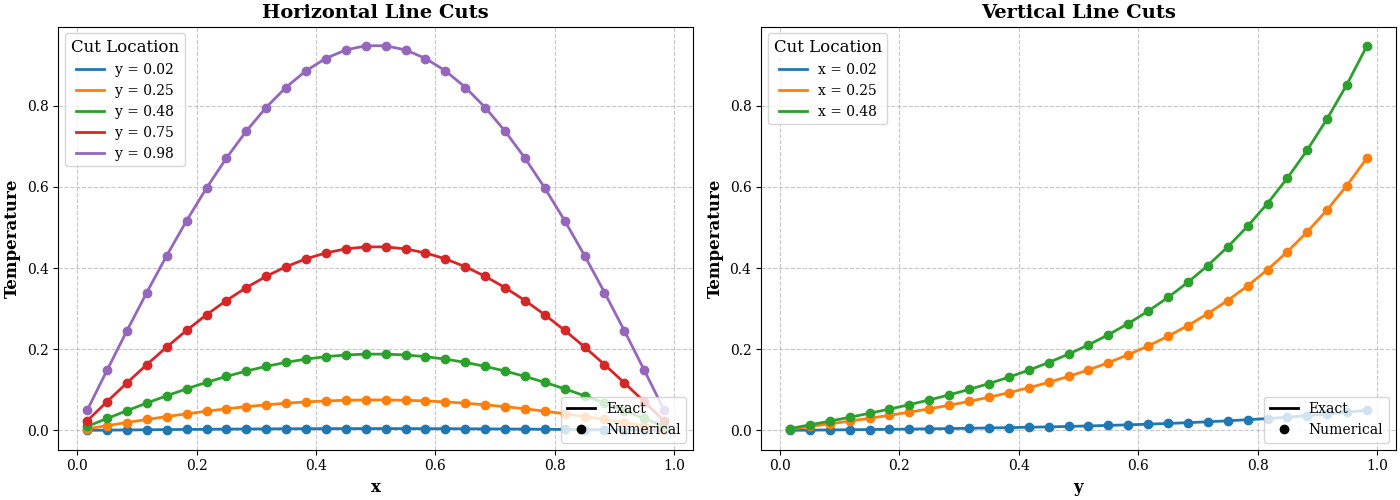
\includegraphics[width=\textwidth]{figures/line_cuts.png}
    \caption{Comparison of numerical and analytical temperature profiles along selected horizontal and vertical line cuts.}
    \label{fig:linecuts}
\end{figure}

\section{Conclusion}

A two-dimensional finite-volume solver for the steady-state heat conduction equation was successfully developed and verified. The governing Laplace equation was discretized using a second-order finite-volume formulation on a structured Cartesian mesh and solved iteratively using the Point Gauss-Seidel method. Dirichlet boundary conditions were implemented through ghost cells, allowing a uniform discretization to be applied throughout the computational domain.

Verification was performed by comparing the numerical solution with the analytical solution of the Laplace equation. Excellent agreement was observed in the temperature contours, line-cut comparisons, and error distribution, while the residual histories demonstrated stable and monotonic convergence of the iterative solution procedure. These results confirm the correctness of the governing equation implementation, spatial discretization, boundary-condition treatment, and iterative solver.

Beyond verifying the numerical implementation, this project establishes the computational framework for a more comprehensive CFD solver. The modular software structure developed in this work enables straightforward extension to accelerated iterative methods such as Successive Over-Relaxation (SOR), Line Gauss-Seidel, Alternating Direction Implicit (ADI), and multigrid techniques. Future developments will also include grid-convergence studies, performance comparisons among iterative methods, and the extension of the solver to more general transport equations encountered in computational fluid dynamics.

This project therefore serves as the first stage in the development of a robust finite-volume CFD code and provides a verified foundation upon which more advanced numerical methods can be systematically implemented and evaluated.



\appendix

\section{Computational Setup}

All numerical simulations were performed on a single workstation. The hardware configuration is reported to ensure reproducibility of the computational results; however, absolute CPU timing values are system-dependent and should be interpreted accordingly.

\subsection{Hardware Configuration}

The simulations were executed on the following system:

\begin{itemize}
    \item Processor: Intel(R) Core(TM) i7-8550U CPU
    \item Number of physical cores: 4
    \item Logical cores: 8
    \item Memory (RAM): 15.88 GB
    \item Architecture: AMD64
\end{itemize}

\subsection{Software Environment}

\begin{itemize}
    \item Programming language: Python 3.x
    \item Numerical libraries: NumPy
    \item Visualization: Matplotlib
    \item Operating system: Windows
\end{itemize}

\subsection{Timing Methodology}

Execution time was measured using a high-resolution wall-clock timer based on \texttt{time.perf\_counter()}, which provides monotonic timing suitable for performance evaluation of iterative solvers.

Since computational performance depends strongly on hardware architecture, CPU frequency scaling, and system load, timing results are reported for reference only and are not intended for direct cross-machine comparison.

\end{document}